\documentclass[conference]{IEEEtran}
\IEEEoverridecommandlockouts
\usepackage[T1]{fontenc}
\usepackage{cite}
\usepackage{amsmath,amssymb}
\usepackage{graphicx}
\usepackage{booktabs}
\usepackage{multirow}
\usepackage{xcolor}
\usepackage{url}
\usepackage{orcidlink}
\hypersetup{hidelinks}

% ---------------------------------------------------------------------------
% Reviewer mark-up. Clean copy: compile main.tex. Annotated copy: compile
% main_annotated.tex, which sets \annotate to 1 before loading this file.
% R1 blue, R2 green, R3 amber, R4 magenta (same colours as the response note).
\providecommand{\annotate}{0}
\definecolor{rI}{HTML}{1F6FB2}
\definecolor{rII}{HTML}{00B050}
\definecolor{rIII}{HTML}{BF8F00}
\definecolor{rIV}{HTML}{C2185B}
\ifnum\annotate=1
  \newcommand{\rone}[1]{{\color{rI}#1}}
  \newcommand{\rtwo}[1]{{\color{rII}#1}}
  \newcommand{\rthree}[1]{{\color{rIII}#1}}
  \newcommand{\rfour}[1]{{\color{rIV}#1}}
\else
  \newcommand{\rone}[1]{#1}
  \newcommand{\rtwo}[1]{#1}
  \newcommand{\rthree}[1]{#1}
  \newcommand{\rfour}[1]{#1}
\fi

% Confluence header and IEEE copyright footer, first page only
\makeatletter
\def\ps@IEEEtitlepagestyle{%
  \def\@oddhead{\parbox{\textwidth}{\centering\footnotesize
    2027 17th International Conference on Cloud Computing, Data Science \& Engineering (Confluence)}}%
  \def\@evenhead{\@oddhead}%
  \def\@oddfoot{\parbox{\textwidth}{\footnotesize 979-8-3195-3311-1/27/\$31.00~\copyright2027 IEEE\hfill}}%
  \def\@evenfoot{\@oddfoot}}
\makeatother

\begin{document}

\title{Repeatability-Calibrated EMG-Kinematic Discordance in Pediatric Gait: A Cross-Sectional and Longitudinal Pilot Study with Wearable Sensors}

\author{
\IEEEauthorblockN{
Deepinder Singh\IEEEauthorrefmark{1}\,\orcidlink{0009-0005-7238-3930},
Vishwanath Bijalwan\IEEEauthorrefmark{1}\,\orcidlink{0000-0002-8661-5430},
Komal\IEEEauthorrefmark{1},\\
Youngshik Kim\IEEEauthorrefmark{2},
Vijay Bhaskar Semwal\IEEEauthorrefmark{3}\,\orcidlink{0000-0003-0767-6057}
}
\IEEEauthorblockA{
\IEEEauthorrefmark{1}Amity School of Engineering \& Technology,
Amity University Punjab, Mohali, India\\
\IEEEauthorrefmark{2}Department of Mechanical Engineering,
Hanbat National University, Daejeon, South Korea\\
\IEEEauthorrefmark{3}Maulana Azad National Institute of Technology,
Bhopal, Madhya Pradesh, India\\
Emails: deepinders0627@gmail.com,
vishwanath.bijalwan@gmail.com,\\
gabakomal11@gmail.com, vsemwal@gmail.com
}
\thanks{Corresponding author: Vishwanath Bijalwan\protect\newline(vishwanath.bijalwan@gmail.com).}
}

\maketitle

\begin{abstract}
Clinical gait analysis rarely asks whether kinematic or electromyographic (EMG) deviations exceed measurement variability. This study scores ankle kinematics and area-normalised tibialis anterior and gastrocnemius envelopes by gait phase against a typically developing (TD) reference, calibrates each score with within-session repeatability, and assigns every visit-limb to one of four concordance classes. In the LIVE-GaitNeuroKids wearable dataset (19 children with cerebral palsy (CP), 11 with idiopathic toe walking (ITW) and 22 TD), a strict rule requiring 95\% confidence beyond the TD limit classified 56.5\% of CP visit-limbs as ankle-only abnormal versus 0\% of TD ($p=0.0002$), robust to age matching, pre-treatment visits and phase registration. Under the standard TD 95th-percentile rule, EMG was flagged in 38.7\% (CP) and 38.1\% (ITW) versus 16.3\% (TD), independently of the ankle flag, and on/off timing showed premature gastrocnemius activity. Positive controls showed that whole-phase EMG scores detect only large timing changes.
\end{abstract}

\begin{IEEEkeywords}
cerebral palsy, idiopathic toe walking, surface electromyography, gait analysis, inertial sensors, measurement repeatability
\end{IEEEkeywords}

\section{Introduction}
Cerebral palsy (CP) and idiopathic toe walking (ITW) are common causes of equinus and toe-walking gait in children referred for clinical gait analysis. Treatments such as botulinum toxin injection, nerve ablation and casting aim to change both how the ankle moves and how the calf and shin muscles are activated. Kinematic outcomes are usually summarised with deviation indices such as the Gait Deviation Index and the Gait Profile Score~\cite{schwartz2008gdi,baker2009gps}, and EMG has analogous indices that measure the distance of activation envelopes from a typical reference~\cite{davoudi2025fingerprint}. These measures are, however, usually reported side by side rather than jointly, so the clinically interesting case in which the two modalities disagree is not made explicit.

Disagreement between movement and muscle activation is plausible. In a randomised trial, botulinum toxin with rehabilitation improved gait kinematics in children with CP without improving surface EMG patterns~\cite{vanderhouwen2011btx}, and in a cohort of 51 patients the relation between kinematic abnormality and abnormal activation patterns was not direct~\cite{syczewska2016emg}. Detecting such disagreement in an individual child is difficult because pediatric EMG is variable: within-session waveform variability in children is roughly twice that of adults~\cite{granata2005repeat}, and repeatability baselines are needed before a between-visit change can be called real~\cite{steele2019repeat}. A discordance flag that ignores this variability risks labelling noise as a clinical finding, \rtwo{and one that overcorrects for it can no longer detect real abnormality.}

The LIVE-GaitNeuroKids dataset~\cite{fernandez2026live,zenodo2026live} provides synchronised inertial kinematics and four-channel surface EMG from children with CP, ITW and typically developing (TD) controls, two walking trials per session and repeated clinical assessments around treatment. This makes it possible to calibrate a concordance analysis against measurement error using wearable rather than laboratory instrumentation. The contributions of this paper are:
\begin{itemize}
\item A visit-level, phase-specific four-class concordance analysis of ankle kinematics and lower-leg EMG, \rtwo{with limits calibrated by the standard error of measurement (SEM) and leave-one-out TD false-positive rates reported per modality;}
\item \rtwo{Repeatability of the wearable scores (SEM, intraclass correlation, minimal detectable change, split-half and waveform estimates), positive controls of EMG sensitivity and} \rthree{EMG on/off timing measures,} to the authors' knowledge the first such analysis on LIVE-GaitNeuroKids;
\item \rtwo{A joint analysis of the ankle and EMG flags} and \rone{a treatment-cycle-aware pilot that judges change against between-session measurement error.}
\end{itemize}

\section{Related Work}
\textbf{Gait deviation indices.} The Gait Deviation Index and Gait Profile Score summarise kinematic distance from a TD reference~\cite{schwartz2008gdi,baker2009gps}. EMG analogues include the Kerpape-Rennes EMG-based gait index and the EMG Profile Score, the latter being a mean per-muscle root mean square error (RMSE) from TD envelopes, and synergy-based dynamic motor control indices~\cite{davoudi2025fingerprint,schwartz2016dmc}. The per-muscle RMSE used here is closely related to the EMG Profile Score; the novelty lies in the joint classification and its calibration, not in the score itself.

\textbf{EMG and kinematics after treatment.} Kinematic improvement without EMG pattern change after botulinum toxin~\cite{vanderhouwen2011btx}, an indirect relation between EMG and kinematic abnormality~\cite{syczewska2016emg}, and systematic post-surgical EMG change despite stable motor-control indices~\cite{davoudi2025fingerprint} all motivate analysing the two modalities jointly.

\textbf{Repeatability.} Within-session EMG variability in healthy children exceeds adult values~\cite{granata2005repeat}, and inter-visit EMG repeatability in CP is comparable to that of unimpaired individuals~\cite{steele2019repeat}. The SEM and minimal detectable change are the usual tools for separating real change from measurement error~\cite{weir2005icc}, \rtwo{and waveform similarity is commonly summarised by the coefficient of multiple correlation (CMC)~\cite{kadaba1989repeat}.}

\textbf{Muscle activation patterns in toe walking.} Premature swing-phase gastrocnemius activity has been reported in both mild diplegic CP and ITW~\cite{policy2001itw}, and botulinum toxin can normalise ankle EMG timing in ITW~\cite{brunt2004itw}.

\section{Materials and Methods}
Fig.~\ref{fig:pipeline} summarises the analysis pipeline.

\begin{figure*}[t]
\centering
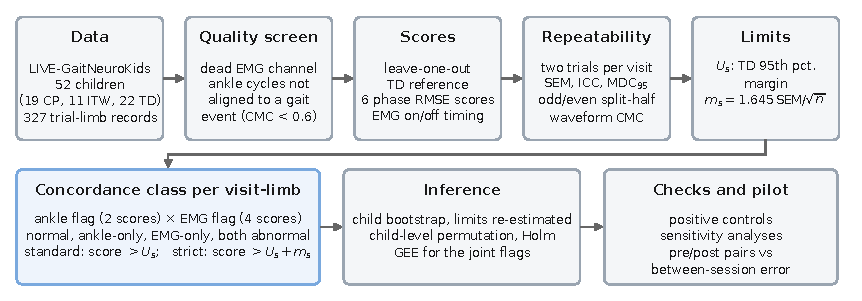
\includegraphics[width=0.86\textwidth]{figs/fig_pipeline.pdf}
\caption{Analysis pipeline. Six phase-specific scores are compared with a leave-one-out TD normal limit $U_s$; the strict rule adds the measurement error of the visit mean, $m_s$. Each visit-limb is assigned to one of four classes under both rules.}
\label{fig:pipeline}
\end{figure*}

\subsection{Dataset, Cohort and Quality Screen}
Version 1.1 of the public LIVE-GaitNeuroKids dataset (Zenodo, CC BY 4.0)~\cite{fernandez2026live,zenodo2026live} was used. Kinematics were recorded with a lower-body inertial system at 100\,Hz and surface EMG from bilateral tibialis anterior (TA) and medial gastrocnemius (GM) placed following SENIAM~\cite{hermens2000seniam}. The providers band-pass filtered (20--400\,Hz), rectified and low-pass filtered (6\,Hz) the EMG, synchronised it with the kinematics, segmented gait cycles and resampled each to 101 samples, with per-sample support (foot contact) labels. Each session contains two walking trials over a 12\,m path. CP and ITW children were assessed immediately before treatment (T0), 1--2 weeks after (T1) and about three months after (T2). Only these processed cycles were used.

\rfour{The dataset lists 59 children (22 CP, 12 ITW, 25 TD). Four (three CP, one ITW) have no processed gait files; for the CP children the participant file notes unavailable video or inertial data, and their ages (7.0--13.4\,y) lie within the analysed range. The 179 trial files gave 358 trial-limb records, of which 19 came from kinematic files containing one leg only and were excluded.} \rone{A quality screen then removed one essentially flat GM channel (amplitude below 5\% of the muscle median) and 12 trial-limb records whose ankle cycles were not aligned to a gait event, detected as a cycle-to-cycle CMC below 0.6; these included every record of three TD children whose cycles started at arbitrary points of the stride.} \rtwo{The analysis therefore used 327 records from 52 children (Table~\ref{tab:cohort}).}

\rtwo{A \emph{visit-limb} is one limb of one child at one visit, with scores averaged over that visit's trials.} For hemiparetic and monoparetic CP only the affected limb was classified; both limbs were classified for diparetic CP, ITW and TD. \rthree{Of 176 visit-limbs, 147 were classified (CP 62, ITW 42, TD 43), 22 of them with a single usable trial. Repeatability used the 146 visit-limbs with two trials, including the unaffected CP limbs (CP 74, ITW 31, TD 41), which is why the two sets differ.}

\begin{table}[t]
\centering
\caption{\rtwo{Analysed cohort. Age at the first analysed visit. $^a$One TD child has no participant record}}
\label{tab:cohort}
\footnotesize
\setlength{\tabcolsep}{4pt}
\rtwo{\begin{tabular}{lccc}
\toprule
 & CP & ITW & TD \\
\midrule
Children analysed & 19 & 11 & 22 \\
Age, y, mean (SD) & 10.2 (3.0) & 9.3 (2.4) & 8.4 (2.2)$^a$ \\
Male/female & 15/4 & 8/3 & 12/9$^a$ \\
Visits per child, median [range] & 2 [1--5] & 2 [1--3] & 1 [1--1] \\
Visit-limbs: classified / repeatability & 62 / 74 & 42 / 31 & 43 / 41 \\
\midrule
\multicolumn{4}{l}{CP subtype: hemiparesis 9, diparesis 9, monoparesis 1;} \\
\multicolumn{4}{l}{GMFCS not recorded. Botulinum toxin: CP 16, ITW 10;} \\
\multicolumn{4}{l}{nerve ablation: CP 5; casting: ITW 2; Achilles tenotomy: ITW 1} \\
\bottomrule
\end{tabular}
}
\end{table}

\subsection{Signal Processing and Phase-Specific Scores}
For each trial and limb the sagittal ankle angle and the TA and GM envelopes were used. Each EMG cycle $e(t)$ was divided by its area, $\tilde e(t)=101\,e(t)/\sum_t e(t)$, so that 1.0 equals the cycle-mean activation and only the shape (timing) of activation is compared. Cycles were averaged within a trial. The stance/swing boundary was set per trial-limb to the median first sample at which the support label switched from contact to no contact. \rtwo{In TD this toe-off lay at 51\% of the cycle, with 98\% of TD cycles within 43--60\%; trials contained a median of 9--11 cycles per group (range 1--49).}

A mean waveform was computed for each TD child over all trials and limbs, and the reference was the unweighted mean across children (Fig.~\ref{fig:wave}). For channel $c\in\{\text{ankle},\text{TA},\text{GM}\}$ and phase $\phi\in\{\text{stance},\text{swing}\}$ the deviation score is
\begin{equation}
d_{c,\phi}=\sqrt{\frac{1}{|\phi|}\sum_{t\in\phi}\big(x_c(t)-r_c(t)\big)^2},
\end{equation}
giving six scores per trial-limb (ankle in degrees, EMG in units of cycle-mean activation). TD children were scored against a leave-one-out reference that excludes them. \rtwo{In a \emph{shape-only ankle} analysis each ankle curve and the reference were mean-centred before scoring, which separates the mean ankle posture from the shape of the curve. The release contains no static calibration trial, so a constant sensor offset cannot be distinguished from a real equinus posture.}

\begin{figure*}[t]
\centering
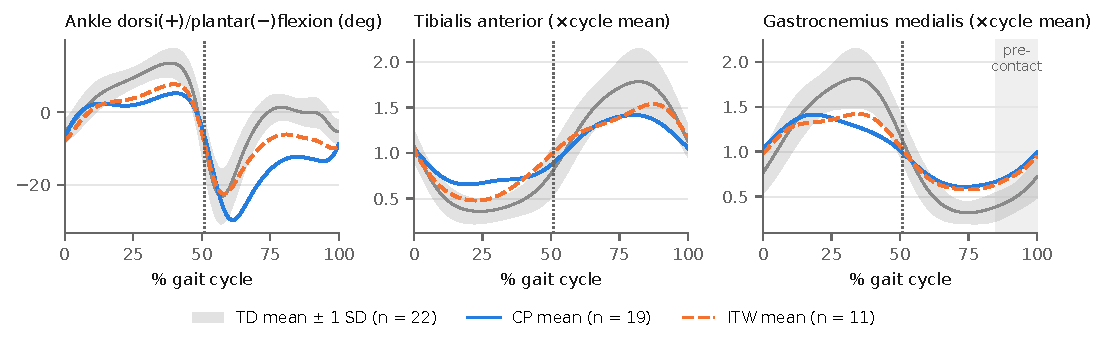
\includegraphics[width=0.92\textwidth]{figs/fig_waveforms.pdf}
\caption{\rtwo{TD reference (line: mean of per-child means; band: $\pm1$ SD between children) with the CP and ITW group means. Dotted line: TD toe-off (51\%); shaded: pre-contact window (85--100\%). EMG is area-normalised so that 1.0 is the cycle-mean activation.}}
\label{fig:wave}
\end{figure*}

\subsection{Repeatability}
\rtwo{For every visit-limb with two trials, let $\Delta_s$ be the difference of score $s$ between the first two trials. Over all such visit-limbs,
\begin{equation}
\mathrm{SEM}_s=\sqrt{\overline{\Delta_s^2}/2},\qquad \mathrm{MDC}_{95,s}=1.96\sqrt2\,\mathrm{SEM}_s,
\end{equation}
together with the intraclass correlation ICC(2,1)~\cite{weir2005icc}, pooled and} \rfour{per group}\rtwo{, with child-bootstrap confidence intervals. The submitted threshold $\delta_s$, the 95th percentile of $|\Delta_s|$, is reported for comparison.} \rone{An independent split-half estimate compared the means of odd and even cycles within each trial; the ratio of the between-trial SEM to the SEM predicted from this cycle-to-cycle noise shows whether separate walks differ more than cycles within a walk.} \rtwo{Waveform repeatability was summarised by the CMC across cycles~\cite{kadaba1989repeat} and the RMSE between the two trial means.}

\subsection{Classification Rules}
A visit-limb is ankle-abnormal if either ankle score exceeds its limit and EMG-abnormal if any of the four EMG scores does. Crossing the two flags gives four classes: both normal, ankle-only, EMG-only and both abnormal. Under the \emph{standard} rule the limit is $U_s$, the 95th percentile of TD visit-limb scores, recomputed without the child for TD children. \rtwo{Under the \emph{strict} rule the limit is $U_s+m_s$ with
\begin{equation}
m_s=1.645\,\mathrm{SEM}_s/\sqrt{n},
\end{equation}
where $n$ is the number of trials averaged, so that a flagged visit mean lies beyond $U_s$ with one-sided 95\% confidence.} \rthree{$U_s$ sets specificity, which is reported as the leave-one-out TD flag rate of each rule; $m_s$ adds only the measurement error of the visit mean, and sensitivity is measured with positive controls (Section~\ref{sec:stat}).} \rtwo{The submitted rule, $U_s+\delta_s$, adds the range of single-trial differences on top of a limit that already contains that variability; it is kept as a sensitivity analysis.} \rfour{Because two ankle scores but four EMG scores are tested, the two modalities have different TD flag rates; both are reported, and an equal-rate calibration raised each modality's percentile until both flagged 9.3\% of TD visit-limbs (ankle 96.4th, EMG 97.2nd percentile).}

\subsection{EMG On/Off Timing}
\rthree{To complement whole-phase RMSE, a muscle was taken to be ON in a cycle sample when its normalised envelope exceeded its own cycle mean. Per visit-limb, the percentage of ON samples was computed for TA and GM in stance and swing, for GM in the pre-contact window (85--100\% of the cycle) and for TA in early stance (0--15\%). A timing flag is set when any of the four phase measures lies outside the leave-one-out TD 2.5--97.5th percentile range, or beyond it by $1.645\,\mathrm{SEM}/\sqrt{n}$ (strict).}

\subsection{Statistical Inference, Positive Controls and Sensitivity}
\label{sec:stat}
Class proportions are reported over visit-limbs with 95\% confidence intervals from a cluster bootstrap over children (2000 resamples)~\cite{efron1993bootstrap}; \rtwo{limits and SEM are re-estimated in every resample and bias-corrected percentile intervals are used. Differences from TD are tested with a child-level permutation test (5000 permutations) on the mean of each child's class share; exact $p$-values are $(k+1)/5001$, and Holm's correction~\cite{holm1979} is applied across the four analyses of each outcome and across the 12 timing comparisons.} \rtwo{The association between the flags is described by the observed versus expected number of both-abnormal visit-limbs, Cohen's $\kappa$ and the odds ratio, and modelled with generalised estimating equations (GEE; logit link, exchangeable correlation, child as cluster)~\cite{liang1986gee} of the EMG flag on the ankle flag and group.}

\rtwo{\emph{Positive controls.} Known changes were added to both trials of all 43 TD visit-limbs, which were rescored against the unaltered leave-one-out reference with the limits of the main analysis: TA and GM timing shifts of 2--15\% of the cycle in both directions, phase-specific amplitude scaling ($\times$1.5--$\times$3), whole-cycle amplitude scaling ($\times$2, removed by area normalisation by design) and the average CP or ITW deviation from the TD reference. For the change rule, the same alteration between two visits counts as detected when an EMG score changes by more than $\delta_s$ or by $1.96\,\mathrm{SEM}\sqrt{1/n_1+1/n_2}$.}

\rtwo{\emph{Sensitivity analyses.} The analysis was repeated on patient visits within the TD age range (5.0--12.2\,y),} on pre-treatment (T0) visits only, with shape-only ankle scores, \rfour{with each cycle's stance and swing registered to the TD toe-off by piecewise-linear time warping,} \rtwo{with a fixed 60\% boundary, without trials whose toe-off lay outside 43--60\%, with amplitude scores (raw ankle angle and raw EMG envelopes), with one EMG score per phase (two EMG tests, matching the ankle), with SEM estimated from TD only, and without the child with the largest ankle offset.}

\subsection{Longitudinal Pilot}
Many children were treated more than once and the T0/T1/T2 labels restart with each treatment. Using the treatment dates in the participant records, a T0 was paired with the follow-up (T2, else T1) of the same treatment cycle only when T0 fell between the previous and current treatment and the follow-up between the current and next treatment. \rone{Ankle improvement is a score decrease larger than the MDC$_{95}$ of a difference of visit means; EMG improvement is assessed only in limbs EMG-abnormal at baseline.} \rthree{Because inertial sensors and electrodes are re-applied at each visit, between-session error was estimated from consecutive visits of the untreated limb of hemiparetic and monoparetic CP children and used as a second, between-session MDC$_{95}$.}

\section{Results}
\subsection{Repeatability}
\rone{Table~\ref{tab:rep} gives the repeatability of the six scores. Ankle scores were highly repeatable (ICC 0.92 and 0.97), whereas EMG scores were not (ICC 0.27--0.55).} \rfour{EMG SEM was 0.12--0.14 in TD, 0.15--0.24 in CP and 0.19--0.23 in ITW, in line with the higher variability reported in children~\cite{granata2005repeat}.} \rtwo{MDC$_{95}$ closely matched the submitted $\delta_s$, and for TA stance and GM swing $\delta_s$ exceeded $U_s$ itself (0.62 versus 0.55; 0.66 versus 0.57), which explains why the $U_s+\delta_s$ rule is extremely strict.} \rone{The split-half estimate was high (ICC 0.87--0.99), and the between-trial error was 2.2--4.5 times that predicted from cycle-to-cycle noise, so separate walks differ more than cycles within a walk and the two-trial estimate is the conservative one.} \rtwo{Waveforms were consistent across cycles (median CMC: ankle 0.93, TA 0.85, GM 0.86), with a median between-trial RMSE of 2.5$^\circ$, 0.18 and 0.17.}

\begin{table*}[t]
\centering
\caption{\rtwo{Within-session repeatability (146 visit-limbs, 50 children; 95\% child-bootstrap CI), submitted threshold $\delta_s$, TD normal limit $U_s$ and strict-rule margin $m_s$ for a two-trial visit. EMG in units of cycle-mean activation}}
\label{tab:rep}
\footnotesize
\rtwo{\begin{tabular}{lcccccc}
\toprule
Score & SEM [95\% CI] & ICC [95\% CI] & MDC$_{95}$ & $\delta_s$ & $U_s$ & $m_s$ ($n$=2) \\
\midrule
Ankle stance (deg) & 1.60 [1.31, 1.86] & 0.92 [0.78, 0.95] & 4.44 & 4.69 & 8.53 & 1.87 \\
Ankle swing (deg) & 1.68 [1.40, 1.93] & 0.97 [0.92, 0.98] & 4.67 & 5.19 & 10.66 & 1.96 \\
TA stance & 0.19 [0.15, 0.22] & 0.27 [0.12, 0.43] & 0.52 & 0.62 & 0.55 & 0.22 \\
TA swing & 0.18 [0.15, 0.21] & 0.45 [0.29, 0.60] & 0.50 & 0.66 & 0.84 & 0.21 \\
GM stance & 0.16 [0.13, 0.18] & 0.55 [0.40, 0.68] & 0.43 & 0.50 & 0.80 & 0.18 \\
GM swing & 0.21 [0.17, 0.25] & 0.27 [0.07, 0.51] & 0.59 & 0.66 & 0.57 & 0.25 \\
\bottomrule
\end{tabular}
}
\end{table*}

\subsection{Concordance Classes and Joint Flags}
\rtwo{Fig.~\ref{fig:wave} shows the patient means against the TD band: the CP ankle was more plantarflexed in stance and swing, TA activity in CP was higher in stance and lower in swing, and GM activity in both patient groups stayed above the TD band from mid-swing into the pre-contact window.}

\rfour{Under the standard rule, TD visit-limbs were flagged at 11.6\% (ankle) and 16.3\% (EMG), the false-positive rates of the two modalities (Table~\ref{tab:classes}).} \rtwo{CP visit-limbs were ankle-abnormal in 71.0\%, and EMG flags were raised in 38.7\% of CP and 38.1\% of ITW visit-limbs ($p=0.017$ and $0.029$; Holm 0.061 and 0.079). Both flags occurred together in 29.0\% of CP visit-limbs versus none in TD ($p=0.0004$). Most EMG flags came from TA stance in CP (15 of 24) and from GM swing in ITW (13 of 16).} \rthree{Under the strict rule TD false positives fell to 0\% (ankle) and 2.3\% (EMG).} CP ankle-only abnormality reached 56.5\% versus 0\% in TD (difference +56.5 points, 95\% CI 33.3--79.0, $p=0.0002$, Holm 0.0008), whereas EMG flags fell to 12.9\% (CP) and 14.3\% (ITW) versus 2.3\% ($p=0.057$ and $0.077$). \rtwo{Under the submitted $U_s+\delta_s$ rule no CP or ITW visit-limb was EMG-abnormal.} \rtwo{One-vote-per-child estimates were close to the visit-limb rates (strict CP ankle-only 52.7\%; standard EMG flag CP 39.4\%, ITW 39.2\%, TD 15.9\%), and within TD, age was not associated with any score ($|\rho|\le0.21$, all $p\ge0.37$, 21 children).} \rfour{With an equal 9.3\% TD flag rate per modality, CP ankle-only abnormality was 56.5\% versus 9.3\% ($p=0.0006$) and EMG flags were 24.2\% (CP, $p=0.038$) and 28.6\% (ITW, $p=0.031$).}

\begin{table}[t]
\centering
\caption{Concordance classes and flags (\% of visit-limbs, 95\% child-bootstrap CI). $n$: visit-limbs/children. Std.: score $>U_s$; Strict: score $>U_s+m_s$. \rthree{Timing flag: Section~III-E.} \rtwo{Rounded classes may not sum to 100}}
\label{tab:classes}
\scriptsize
\setlength{\tabcolsep}{2.2pt}
\resizebox{\columnwidth}{!}{\rtwo{\begin{tabular}{llccc}
\toprule
Rule & Class & CP ($n$=62/19) & ITW ($n$=42/11) & TD ($n$=43/22) \\
\midrule
\multirow{7}{*}{Std.} & Both normal & 19.4 [6.0, 42.5] & 52.4 [36.8, 78.1] & 72.1 [61.9, 86.0] \\
 & Ankle-only & \textbf{41.9} [18.9, 74.6] & 9.5 [0.0, 23.5] & 11.6 [0.0, 20.5] \\
 & EMG-only & 9.7 [1.5, 27.9] & 28.6 [16.2, 52.8] & 16.3 [6.8, 26.2] \\
 & Both abn. & 29.0 [3.9, 53.3] & 9.5 [0.0, 24.4] & 0.0 [0.0, 4.5] \\
\cmidrule(l){2-5}
 & Ankle flag & 71.0 [46.3, 87.8] & 19.0 [2.2, 35.9] & 11.6 [6.8, 17.7] \\
 & EMG flag & 38.7 [7.6, 64.3] & 38.1 [16.3, 57.5] & 16.3 [6.8, 25.6] \\
 & Timing flag & 50.0 & 45.2 & 18.6 \\
\midrule
\multirow{7}{*}{Strict} & Both normal & 30.6 [13.2, 53.8] & 83.3 [63.8, 100.0] & 97.7 [93.0, 100.0] \\
 & Ankle-only & \textbf{56.5} [30.8, 77.0] & 2.4 [0.0, 11.8] & 0.0 [0.0, 4.5] \\
 & EMG-only & 6.5 [0.0, 22.6] & 14.3 [1.9, 35.4] & 2.3 [0.0, 7.0] \\
 & Both abn. & 6.5 [0.0, 21.6] & 0.0 [0.0, 3.1] & 0.0 [0.0, 0.0] \\
\cmidrule(l){2-5}
 & Ankle flag & 62.9 [38.5, 82.6] & 2.4 [0.0, 12.2] & 0.0 [0.0, 4.5] \\
 & EMG flag & 12.9 [0.0, 34.0] & 14.3 [0.0, 35.8] & 2.3 [0.0, 7.0] \\
 & Timing flag & 12.9 & 11.9 & 2.3 \\
\bottomrule
\end{tabular}
}}
\end{table}

\rtwo{The two flags were independent. In CP, 18 visit-limbs were both abnormal against 17.0 expected under independence ($\kappa=0.06$; odds ratio 1.34, 95\% CI 0.38--7.14). In the GEE, the ankle flag did not predict the EMG flag (OR 1.28, $p=0.62$), whereas group did (ITW versus TD OR 3.11, 95\% CI 1.22--7.92, $p=0.017$; CP OR 2.80, $p=0.089$).}

\subsection{Sensitivity Analyses}
\rtwo{CP ankle-only abnormality under the strict rule exceeded TD in every analysis (Fig.~\ref{fig:forest}; all $p=0.0002$): age-matched 62.0\% versus 0\%, pre-treatment 46.4\% versus 0\%, shape-only ankle 51.6\% versus 4.7\%,} \rfour{toe-off registered 48.4\% versus 4.7\%,} \rtwo{fixed 60\% boundary +57.4 points, without extreme toe-offs +53.4, amplitude scores +59.7, two EMG tests +59.7, TD-only SEM 54.8\% versus 2.3\% and without the child with the largest offset +50.0.} \rone{With the submitted rule, shape-only CP ankle-only abnormality was 33.9\%; the 12.9\% reported in the submitted version resulted from the misaligned TD cycles, which widened the TD shape limits.} \rfour{Registration also increased the standard-rule CP EMG flag difference to +30.5 points ($p=0.004$).} \rtwo{The ITW EMG flag stayed 14--25 points above TD under the standard rule in every analysis; under the strict rule it differed from TD only with the fixed boundary ($p=0.037$) and TD-only SEM ($p=0.019$), uncorrected.} \rfour{The extreme toe-off values of 35\% and 81\% came from trials with one and two usable cycles; 12 trial-limbs from five children (11 CP, 1 ITW) lay outside 43--60\%.}

\begin{figure}[t]
\centering
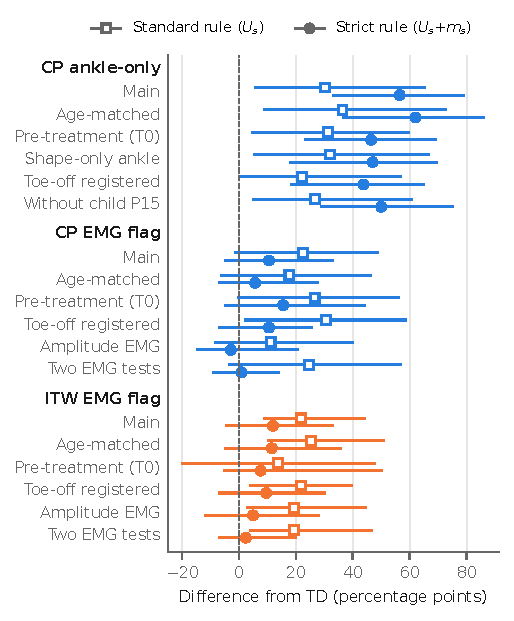
\includegraphics[width=0.94\columnwidth]{figs/fig_forest.pdf}
\caption{\rtwo{Difference from TD in percentage points (95\% child-bootstrap CI) for the main and sensitivity analyses, under the standard (open squares) and strict (filled circles) rules.}}
\label{fig:forest}
\end{figure}

\subsection{Positive Controls}
\rtwo{Table~\ref{tab:controls} shows how often known changes were detected. A 15\% timing shift was flagged in 63--79\% of TD visit-limbs at $U_s$, 35--37\% under the strict rule and 0--5\% at $U_s+\delta_s$; tripling TA stance or GM swing activity was flagged in 65\%, 42--47\% and 0\%. Adding the average CP or ITW EMG deviation raised the standard-rule flag rate only from 16\% to 30\% and 21\%. Whole-cycle amplitude changes were invisible, as intended. As a change rule, $\delta_s$ detected at most 26\% of 15\% shifts and the within-session MDC$_{95}$ 51--60\% of large changes.} \rthree{The strict rule thus keeps TD false positives at 2.3\% while detecting large EMG changes in 35--47\% of limbs,} \rtwo{whereas the submitted $U_s+\delta_s$ rule could essentially never flag EMG.}

\begin{table}[t]
\centering
\caption{\rtwo{Positive controls: \% of 43 TD visit-limbs flagged (EMG flag; $^b$ankle flag) after a known change. Ranges: muscles and shift directions. $^a$Same change between two visits exceeding the change threshold}}
\label{tab:controls}
\scriptsize
\setlength{\tabcolsep}{3pt}
\rtwo{\begin{tabular}{lccccc}
\toprule
 & \multicolumn{3}{c}{Visit flagged} & \multicolumn{2}{c}{Change detected$^a$} \\
\cmidrule(lr){2-4}\cmidrule(lr){5-6}
Change added to TD data & $U_s$ & Strict & $U_s{+}\delta_s$ & $\delta_s$ & MDC$_{95}$ \\
\midrule
No change (false-alarm rate) & 16 & 2 & 0 & 0 & 0 \\
Timing shift 10\% (TA+GM) & 42--63 & 12--14 & 0 & 0 & 19--28 \\
Timing shift 15\% (TA+GM) & 63--79 & 35--37 & 0--5 & 5--26 & 51--56 \\
GM swing activity $\times$3 & 65 & 42 & 0 & 0 & 51 \\
TA stance activity $\times$3 & 65 & 47 & 0 & 2 & 60 \\
Whole-cycle amplitude $\times$2 & 16 & 2 & 0 & 0 & 0 \\
Average CP EMG deviation & 30 & 7 & 0 & 0 & 0 \\
Average ITW EMG deviation & 21 & 7 & 0 & 0 & 0 \\
Average CP ankle deviation$^b$ & 81 & 60 & 26 & -- & -- \\
\bottomrule
\end{tabular}
}
\end{table}

\subsection{EMG Timing}
\rthree{GM was active before initial contact in CP and ITW (median 12.5\% and 9.4\% of the pre-contact window versus 0\% in TD; +18.6 and +16.6 points, Holm $p=0.013$ and $0.007$) and more active in swing (+11.1 and +9.4 points; Holm $p=0.017$ and $0.013$). In CP, TA activity shifted from swing ($-$11.1 points, Holm $p=0.007$) to stance (+14.6, Holm $p=0.008$). Timing flags were raised in 50.0\% (CP) and 45.2\% (ITW) versus 18.6\% (TD) of visit-limbs ($p=0.004$ and $0.017$); under the strict margin 12.9\% and 11.9\% versus 2.3\% ($p=0.044$ and $0.062$).} \rtwo{Premature GM activity persisted on pre-treatment visits (CP $p=0.002$; ITW, five children, $p=0.026$) and age-matched visits ($p=0.003$ and $0.001$).} \rthree{The timing measures were themselves noisy within a session (ICC 0.44--0.59, SEM 15--23 points).}

\subsection{Longitudinal Pilot}
\rone{Only seven children had a valid same-cycle pre/post pair (three CP, four ITW; 14 limbs), with follow-up 56--224 days after T0 and 14--131 days after treatment; five pairs used a T1 visit, nominally 1--2 weeks post-treatment.} \rthree{In untreated CP limbs (19 consecutive-visit pairs, 10 children, median 105 days apart) the between-session SEM was 2.6--3.2 times the within-session value for the ankle and 1.2--1.4 times for EMG, giving a between-session MDC$_{95}$ of 8.3$^\circ$ (stance) and 10.4$^\circ$ (swing).} \rone{Ankle improvement exceeded this threshold in both limbs of one CP child and one limb of another. Five limbs were EMG-abnormal at baseline under the standard rule and three under the strict rule; none improved beyond the between-session threshold, and one GM stance improvement ($-0.42$) exceeded the within-session (0.31) but not the between-session MDC$_{95}$ (0.43). Given the positive controls, the absence of detected EMG change is uninformative.}

\section{Discussion}
CP ankle abnormality was the most robust finding: ankle scores were repeatable (ICC above 0.9), and under the strict rule CP ankle-only abnormality stayed 44--62 points above TD in every data subset, phase definition and calibration tested. \rtwo{EMG was different. Whole-phase RMSE of area-normalised envelopes had low repeatability and limited sensitivity, and the submitted $U_s+\delta_s$ rule could not flag EMG at all, so the earlier conclusion that EMG deviations disappear under calibration reflected the rule rather than the children; it is withdrawn.} \rthree{Timing measures, which do not dilute brief events over a whole phase, showed premature GM activity before initial contact in both CP and ITW, consistent with the premature calf firing described in toe walkers~\cite{policy2001itw} and with the timing changes reported after botulinum toxin in ITW~\cite{brunt2004itw}.}

\rtwo{The ankle and EMG flags were independent ($\kappa$ near zero, GEE odds ratio 1.28), so the CP ankle-only class mostly reflects a frequent ankle flag combined with an independent, less frequent EMG flag rather than a specific discordant phenotype.} This agrees with reports that kinematic abnormality in CP is not a direct consequence of abnormal activation patterns~\cite{syczewska2016emg} and that kinematics can improve after botulinum toxin without EMG pattern change~\cite{vanderhouwen2011btx}. \rone{The dataset contains no clinical outcome scores, so the classes are a measurement-level description and their clinical validity remains to be tested.}

\rone{Mean posture and shape must also be separated. An equinus posture is clinically real, but with re-applied inertial sensors and no static calibration it cannot be separated from a sensor offset; the CP ankle finding nevertheless held for curve shape alone.} \rthree{Between-session ankle error was about three times the within-session error, so treatment monitoring with wearable sensors should use shape-based scores and between-session thresholds, ideally from repeated sessions of TD children.} \rtwo{The ITW swing-GM finding and the low treatment sensitivity of EMG remain hypotheses for larger samples.}

\textit{Limitations.} \rone{The cohorts are small, especially ITW and the seven-child pilot, and treatments were heterogeneous.} Only two muscles and one joint were available, \rone{and only two walks per session; more walks would reduce the margin $m_s$.} \rfour{Walking speed and trial duration are not in the release, which contains time-normalised cycles only; slower walking can alter EMG timing and ankle range, so part of the group differences may reflect speed.} \rtwo{GMFCS levels are not recorded,} \rthree{between-session error came from untreated CP limbs rather than TD retests,} \rfour{and although all exclusions were technical and the excluded children's ages lie within the analysed range, selection bias cannot be ruled out if missing data relate to severity.} A flag indicates measurable deviation; it does not establish treatment failure.

\section{Conclusion}
A repeatability-calibrated, phase-specific concordance analysis of wearable gait data showed abnormal ankle kinematics in about half of CP visit-limbs, robust to age matching, pre-treatment visits, curve shape and phase registration. \rtwo{EMG abnormality was elevated in CP and ITW and independent of the ankle flag, and timing measures showed premature gastrocnemius activity, but whole-phase scores of area-normalised envelopes detected only large changes.} \rthree{Before EMG is used to track pediatric treatment response, studies should record more walks per session, estimate between-session error in typically developing children and use timing-specific measures.} \rtwo{The analysis code, score distributions, the pilot table and the list of excluded records} are publicly available at \url{https://github.com/deepindersinghbti/pediatric-gait-discordance}.

\begin{thebibliography}{00}
\bibitem{schwartz2008gdi} M. H. Schwartz and A. Rozumalski, ``The gait deviation index: A new comprehensive index of gait pathology,'' \emph{Gait Posture}, vol. 28, no. 3, pp. 351--357, 2008.
\bibitem{baker2009gps} R. Baker \emph{et al.}, ``The gait profile score and movement analysis profile,'' \emph{Gait Posture}, vol. 30, no. 3, pp. 265--269, 2009.
\bibitem{davoudi2025fingerprint} M. Davoudi, F. Salami, R. Reisig, D. A. Patikas, N. A. Beckmann, K. S. Gather, and S. I. Wolf, ``Are electromyography data a fingerprint for patients with cerebral palsy (CP)?'' \emph{Appl. Sci.}, vol. 15, no. 2, Art. no. 766, 2025, doi: 10.3390/app15020766.
\bibitem{vanderhouwen2011btx} L. E. E. van der Houwen \emph{et al.}, ``Botulinum toxin A injections do not improve surface EMG patterns during gait in children with cerebral palsy: A randomized controlled study,'' \emph{Gait Posture}, vol. 33, no. 2, pp. 147--151, 2011.
\bibitem{syczewska2016emg} M. Syczewska and A. \'{S}wi\k{e}cicka, ``Are electromyographic patterns during gait related to abnormality level of the gait in patients with spastic cerebral palsy?'' \emph{Acta Bioeng. Biomech.}, vol. 18, no. 3, pp. 91--96, 2016, doi: 10.5277/ABB-00474-2015-02.
\bibitem{granata2005repeat} K. P. Granata, D. A. Padua, and M. F. Abel, ``Repeatability of surface EMG during gait in children,'' \emph{Gait Posture}, vol. 22, no. 4, pp. 346--350, 2005.
\bibitem{steele2019repeat} K. M. Steele, M. E. Munger, K. M. Peters, B. R. Shuman, and M. H. Schwartz, ``Repeatability of electromyography recordings and muscle synergies during gait among children with cerebral palsy,'' \emph{Gait Posture}, vol. 67, pp. 290--295, 2019.
\bibitem{fernandez2026live} C. Fern\'{a}ndez-Gonz\'{a}lez \emph{et al.}, ``LIVE-GaitNeuroKids: A multimodal and longitudinal gait dataset with inertial, video and surface electromyography in neuromotor conditions and typically developing children,'' \emph{Sci. Data}, 2026, doi: 10.1038/s41597-026-08424-4.
\bibitem{zenodo2026live} C. Fern\'{a}ndez-Gonz\'{a}lez \emph{et al.}, ``LIVE-GaitNeuroKids dataset,'' Zenodo, v1.1, 2026, doi: 10.5281/zenodo.21278362.
\bibitem{schwartz2016dmc} M. H. Schwartz, A. Rozumalski, and K. M. Steele, ``Dynamic motor control is associated with treatment outcomes for children with cerebral palsy,'' \emph{Dev. Med. Child Neurol.}, vol. 58, no. 11, pp. 1139--1145, 2016.
\bibitem{weir2005icc} J. P. Weir, ``Quantifying test-retest reliability using the intraclass correlation coefficient and the SEM,'' \emph{J. Strength Cond. Res.}, vol. 19, no. 1, pp. 231--240, 2005.
\bibitem{kadaba1989repeat} M. P. Kadaba, H. K. Ramakrishnan, M. E. Wootten, J. Gainey, G. Gorton, and G. V. B. Cochran, ``Repeatability of kinematic, kinetic, and electromyographic data in normal adult gait,'' \emph{J. Orthop. Res.}, vol. 7, no. 6, pp. 849--860, 1989.
\bibitem{policy2001itw} J. F. Policy, L. Torburn, L. A. Rinsky, and J. Rose, ``Electromyographic test to differentiate mild diplegic cerebral palsy and idiopathic toe-walking,'' \emph{J. Pediatr. Orthop.}, vol. 21, no. 6, pp. 784--789, 2001.
\bibitem{brunt2004itw} D. Brunt, R. Woo, H. D. Kim, M. S. Ko, C. Senesac, and S. Li, ``Effect of botulinum toxin type A on gait of children who are idiopathic toe-walkers,'' \emph{J. Surg. Orthop. Adv.}, vol. 13, no. 3, pp. 149--155, 2004.
\bibitem{hermens2000seniam} H. J. Hermens, B. Freriks, C. Disselhorst-Klug, and G. Rau, ``Development of recommendations for SEMG sensors and sensor placement procedures,'' \emph{J. Electromyogr. Kinesiol.}, vol. 10, no. 5, pp. 361--374, 2000.
\bibitem{efron1993bootstrap} B. Efron and R. J. Tibshirani, \emph{An Introduction to the Bootstrap}. New York, NY, USA: Chapman \& Hall, 1993.
\bibitem{holm1979} S. Holm, ``A simple sequentially rejective multiple test procedure,'' \emph{Scand. J. Statist.}, vol. 6, no. 2, pp. 65--70, 1979.
\bibitem{liang1986gee} K.-Y. Liang and S. L. Zeger, ``Longitudinal data analysis using generalized linear models,'' \emph{Biometrika}, vol. 73, no. 1, pp. 13--22, 1986.
\end{thebibliography}

\end{document}
